% Options for packages loaded elsewhere
\PassOptionsToPackage{unicode}{hyperref}
\PassOptionsToPackage{hyphens}{url}
\PassOptionsToPackage{dvipsnames,svgnames,x11names}{xcolor}
%
\documentclass[
  11pt,
]{article}
\usepackage{amsmath,amssymb}
\usepackage{iftex}
\ifPDFTeX
  \usepackage[T1]{fontenc}
  \usepackage[utf8]{inputenc}
  \usepackage{textcomp} % provide euro and other symbols
\else % if luatex or xetex
  \usepackage{unicode-math} % this also loads fontspec
  \defaultfontfeatures{Scale=MatchLowercase}
  \defaultfontfeatures[\rmfamily]{Ligatures=TeX,Scale=1}
\fi
\usepackage{lmodern}
\ifPDFTeX\else
  % xetex/luatex font selection
\fi
% Use upquote if available, for straight quotes in verbatim environments
\IfFileExists{upquote.sty}{\usepackage{upquote}}{}
\IfFileExists{microtype.sty}{% use microtype if available
  \usepackage[]{microtype}
  \UseMicrotypeSet[protrusion]{basicmath} % disable protrusion for tt fonts
}{}
\makeatletter
\@ifundefined{KOMAClassName}{% if non-KOMA class
  \IfFileExists{parskip.sty}{%
    \usepackage{parskip}
  }{% else
    \setlength{\parindent}{0pt}
    \setlength{\parskip}{6pt plus 2pt minus 1pt}}
}{% if KOMA class
  \KOMAoptions{parskip=half}}
\makeatother
\usepackage{xcolor}
\usepackage[margin=22mm]{geometry}
\usepackage{longtable,booktabs,array}
\usepackage{calc} % for calculating minipage widths
% Correct order of tables after \paragraph or \subparagraph
\usepackage{etoolbox}
\makeatletter
\patchcmd\longtable{\par}{\if@noskipsec\mbox{}\fi\par}{}{}
\makeatother
% Allow footnotes in longtable head/foot
\IfFileExists{footnotehyper.sty}{\usepackage{footnotehyper}}{\usepackage{footnote}}
\makesavenoteenv{longtable}
\usepackage{graphicx}
\makeatletter
\def\maxwidth{\ifdim\Gin@nat@width>\linewidth\linewidth\else\Gin@nat@width\fi}
\def\maxheight{\ifdim\Gin@nat@height>\textheight\textheight\else\Gin@nat@height\fi}
\makeatother
% Scale images if necessary, so that they will not overflow the page
% margins by default, and it is still possible to overwrite the defaults
% using explicit options in \includegraphics[width, height, ...]{}
\setkeys{Gin}{width=\maxwidth,height=\maxheight,keepaspectratio}
% Set default figure placement to htbp
\makeatletter
\def\fps@figure{htbp}
\makeatother
\setlength{\emergencystretch}{3em} % prevent overfull lines
\providecommand{\tightlist}{%
  \setlength{\itemsep}{0pt}\setlength{\parskip}{0pt}}
\setcounter{secnumdepth}{-\maxdimen} % remove section numbering
\ifLuaTeX
\usepackage[bidi=basic]{babel}
\else
\usepackage[bidi=default]{babel}
\fi
\babelprovide[main,import]{french}
% get rid of language-specific shorthands (see #6817):
\let\LanguageShortHands\languageshorthands
\def\languageshorthands#1{}
\ifLuaTeX
  \usepackage{selnolig}  % disable illegal ligatures
\fi
\IfFileExists{bookmark.sty}{\usepackage{bookmark}}{\usepackage{hyperref}}
\IfFileExists{xurl.sty}{\usepackage{xurl}}{} % add URL line breaks if available
\urlstyle{same}
\hypersetup{
  pdftitle={Corrélations ancrées, carte d'identité et réduction énergétique},
  pdfauthor={Vincent P. P. NOËL - dossier de recherche, rédaction assistée},
  pdflang={fr},
  colorlinks=true,
  linkcolor={Maroon},
  filecolor={Maroon},
  citecolor={Blue},
  urlcolor={Blue},
  pdfcreator={LaTeX via pandoc}}

\title{Corrélations ancrées, carte d'identité et réduction énergétique}
\usepackage{etoolbox}
\makeatletter
\providecommand{\subtitle}[1]{% add subtitle to \maketitle
  \apptocmd{\@title}{\par {\large #1 \par}}{}{}
}
\makeatother
\subtitle{Note de recherche - V6.54 - Identité arithmétique et énergie
globale}
\author{Vincent P. P. NOËL - dossier de recherche, rédaction assistée}
\date{14 octobre 2026}

\begin{document}
\maketitle

\hypertarget{la-question-et-le-ruxe9sultat-de-cette-passe}{%
\section{La question et le résultat de cette
passe}\label{la-question-et-le-ruxe9sultat-de-cette-passe}}

Les trois idées proposées ont des fonctions distinctes : identifier
exactement les vrais coefficients premiers ; mesurer leurs fluctuations
sans perdre les coupures ; transférer une borne énergétique en
information sur les zéros.

Le pont retenu est classique : pour les vrais poids de von Mangoldt, la
borne globale \(J(X)=O(X^2)\), où \[
J(X)=\int_1^X(\psi(x)-x)^2\,dx,
\] équivaut à RH. Les corrélations ancrées permettent d'écrire
exactement cette énergie. La carte d'identité garantit que sa
transformée détecte les zéros.

\textbf{Aucune borne globale nouvelle de cette force n'est obtenue.}
Cette note organise une reprise de recherche, avec preuves auxiliaires,
contre-modèles et expériences finies. La réduction est connue ; aucune
priorité n'est revendiquée.

Le corpus récupéré citait déjà Cramér et Brent--Platt--Trudgian dans les
documents 37 et 45. Les théorèmes A et B du dossier utilisent aussi des
moyennes quadratiques, au second ordre. Nous retrouvons donc un fil
existant. Le travail présent précise l'ancrage des corrélations et le
rôle indispensable de l'identité arithmétique ; il ne fournit pas
l'estimation qui manquait à ce fil.

\begin{figure}
\centering
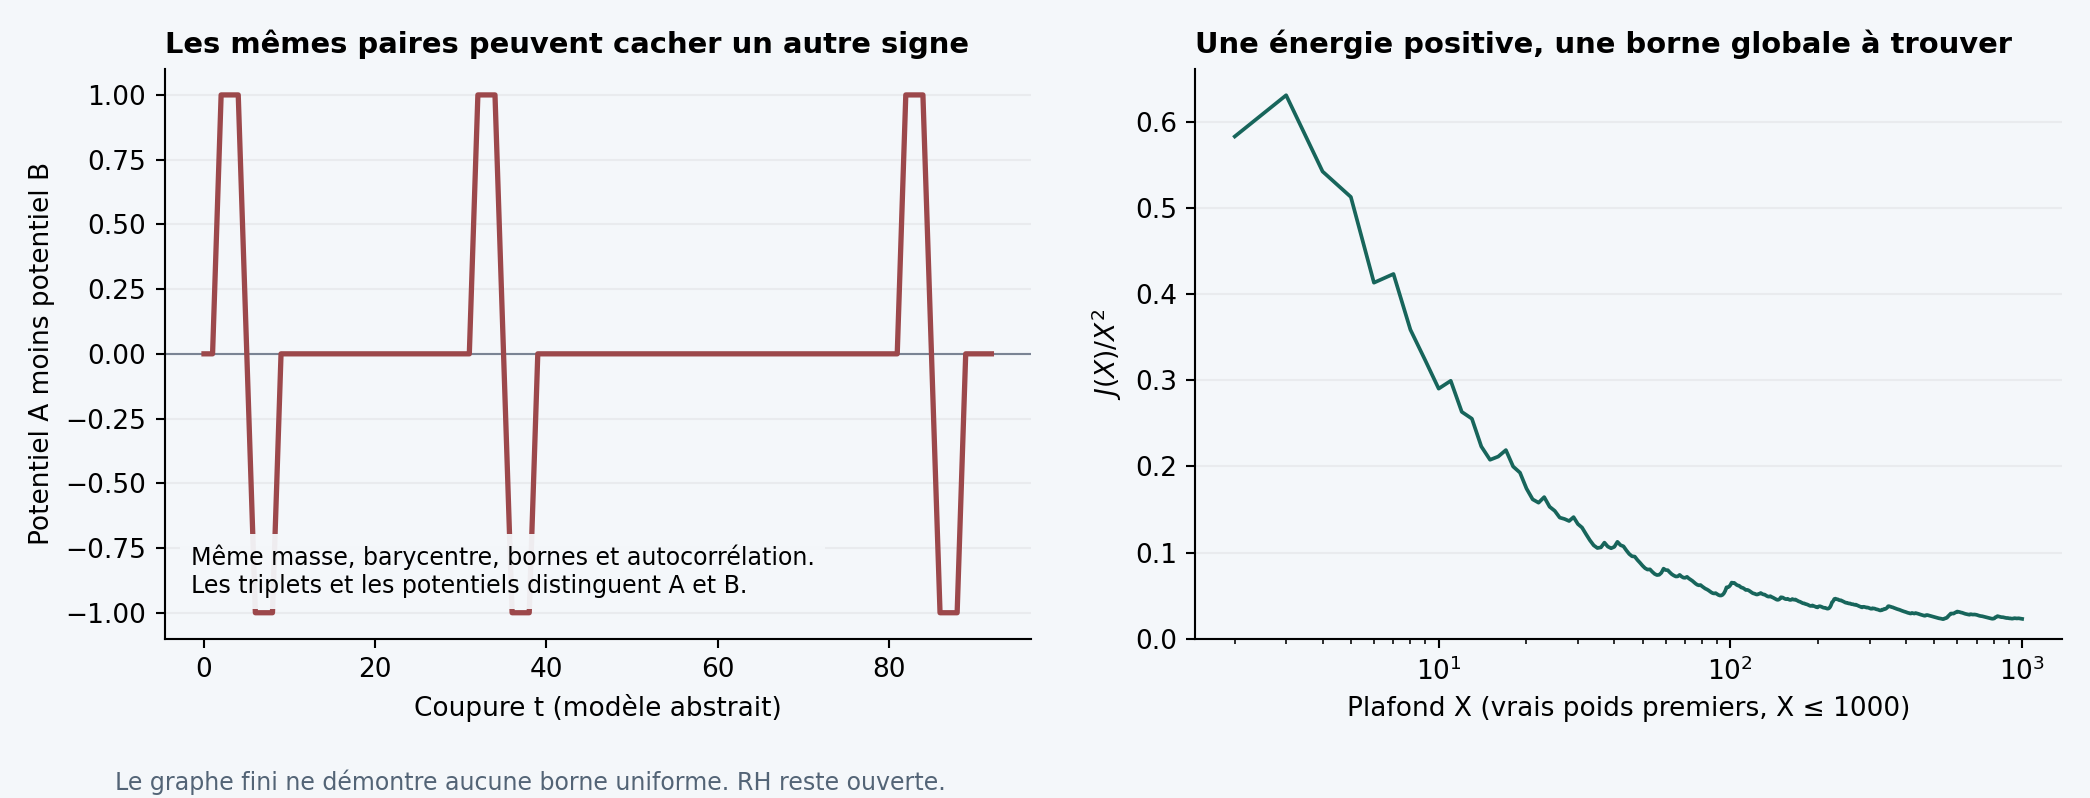
\includegraphics{CORRELATIONS_VISUEL.png}
\caption{L'autocorrélation ordinaire peut perdre le signe ; l'énergie
ancrée donne une autre obligation globale.}
\end{figure}

\hypertarget{les-deux-uxe9luxe9ments-repris-dans-v6.54}{%
\subsection{Les deux éléments repris dans
V6.54}\label{les-deux-uxe9luxe9ments-repris-dans-v6.54}}

\textbf{Type de document :} note de recherche et dossier de preuves
auxiliaires, accompagnés des programmes, résultats et audits. Le critère
énergétique et l'identité de diviseurs sont classiques ; aucune preuve
nouvelle de RH n'est revendiquée.

\begin{longtable}[]{@{}
  >{\raggedright\arraybackslash}p{(\columnwidth - 4\tabcolsep) * \real{0.3333}}
  >{\raggedright\arraybackslash}p{(\columnwidth - 4\tabcolsep) * \real{0.3333}}
  >{\raggedright\arraybackslash}p{(\columnwidth - 4\tabcolsep) * \real{0.3333}}@{}}
\toprule\noalign{}
\begin{minipage}[b]{\linewidth}\raggedright
Élément
\end{minipage} & \begin{minipage}[b]{\linewidth}\raggedright
Travail écrit et exécuté
\end{minipage} & \begin{minipage}[b]{\linewidth}\raggedright
Obligation restante
\end{minipage} \\
\midrule\noalign{}
\endhead
\bottomrule\noalign{}
\endlastfoot
Carte d'identité des vrais poids premiers & Preuve de l'identité de
diviseurs, unicité, inversion de Möbius et contrôle exact jusqu'à 1000 ;
contre-modèle qui explique son rôle indispensable. & L'identité ne donne
pas une estimation quantitative des fluctuations. \\
Énergie ancrée J & Développement exact en corrélations, critère
classique de Cramér, preuve du sens borne vers RH, bilan logarithmique ;
calculs recoupés à 85 et 90 chiffres. & Établir une constante
indépendante de X dans la borne quadratique globale. \\
\end{longtable}

Les deux éléments sont reliés par \(-\zeta'/\zeta\). L'identité
identifie cette série de Dirichlet ; la borne d'énergie donnerait
l'holomorphie qui exclut les zéros à droite de la ligne critique, comme
le détaille la preuve du §4. Le critère de Weil donnerait alors la
positivité sur tous les tests admissibles.

La passe a d'abord été livrée sous le nom « complément V6.53 » ; V6.54
corrige ce suivi éditorial. Les journaux de calcul originaux et leurs
audits sont conservés avec leur provenance, sans nouveau calcul
scientifique prétendu.

\hypertarget{des-statistiques-qui-conservent-linformation-utile}{%
\section{1. Des statistiques qui conservent l'information
utile}\label{des-statistiques-qui-conservent-linformation-utile}}

Un poids \(\Lambda(n)\) vaut \(\log p\) si \(n=p^k\), et zéro sinon. La
fonction \(\psi(x)=\sum_{n\le x}\Lambda(n)\) cumule ces poids. Son écart
à la densité moyenne est \(E(x)=\psi(x)-x\).

L'énergie \(J\) est positive par définition, quel que soit le signe de
\(E\). Son intérêt pour RH vient d'une limite de croissance, pas de
cette positivité.

\textbf{Identité de corrélation ancrée.} Pour tout \(X\ge1\), \[
\begin{aligned}
J(X)={}&\sum_{m,n\le X}\Lambda(m)\Lambda(n)(X-\max(m,n))\\
&-\sum_{n\le X}\Lambda(n)(X^2-n^2)+\frac{X^3-1}{3}.
\end{aligned}
\] \textbf{Preuve.} Développer \((\psi(x)-x)^2\), puis intégrer les
indicatrices \(\mathbf1_{x\ge n}\). Les conventions aux entiers
n'affectent pas l'intégrale. Le noyau quadratique est un Gram : \[
X-\max(m,n)=\int_1^X\mathbf1_{x\ge m}\mathbf1_{x\ge n}\,dx.
\] Il conserve les positions absolues et le plafond. La somme
quadratique positive ne domine pas automatiquement le terme croisé. Les
trois grandes contributions, de taille \(X^3\), doivent se compenser
jusqu'à une énergie \(O(X^2)\).

On peut aussi séparer la diagonale et les décalages : \[
\sum_{m,n\le X}\Lambda(m)\Lambda(n)(X-\max(m,n))
=\sum_{n\le X}\Lambda(n)^2(X-n)
+2\sum_{h\ge1}\sum_{n\le X-h}\Lambda(n)\Lambda(n+h)(X-n-h).
\] Une information moyenne sur les paires doit contrôler précisément ces
poids et les erreurs restantes pour servir à la borne globale.

\hypertarget{pourquoi-les-corruxe9lations-par-uxe9carts-ne-suffisent-pas}{%
\section{2. Pourquoi les corrélations par écarts ne suffisent
pas}\label{pourquoi-les-corruxe9lations-par-uxe9carts-ne-suffisent-pas}}

Voici un modèle exact, construit par convolution de petites briques : \[
P=\{0,30,80\},\quad Q=\{0,1,6,8,10\},\quad Q'=10-Q,
\quad A=P+Q,\quad B=P+Q'.
\] Toutes les sommes sont distinctes. Les deux configurations ont 15
points, un premier moment 625, les mêmes bornes 0 et 90 et exactement
les mêmes différences signées avec multiplicité.

\textbf{Preuve de l'autocorrélation identique.} Pour les mesures de
points, \(\nu_A=\nu_P*\nu_Q\), \(\nu_B=\nu_P*\nu_{Q'}\). La
réflexion-translation \(Q'=10-Q\) conserve l'autocorrélation de \(Q\).
La factorisation \((\nu_P*\nu_Q)*(\check\nu_P*\check\nu_Q)\) donne donc
le résultat. Le barycentre de \(Q\) vaut 5, ce qui conserve aussi le
premier moment.

Pourtant, avec \(P_\nu(t)=\sum_u(t-u)_+\),

\begin{longtable}[]{@{}rrrr@{}}
\toprule\noalign{}
Coupure & \(P_A\) & \(P_B\) & Différence \\
\midrule\noalign{}
\endhead
\bottomrule\noalign{}
\endlastfoot
3 & 5 & 4 & 1 \\
7 & 14 & 15 & -1 \\
\end{longtable}

Avec la même source \(\mu=\nu_A\), le signal associé à A est nul, et
celui associé à B vaut -1 en 7. Une triple corrélation distingue aussi
les modèles : le nombre de triplets \((u,u+1,u+6)\) est 3 pour A et zéro
pour B. Cela vérifie une perte de phase précise ; cela ne prétend pas
identifier les premiers ni donner une propriété universelle de toutes
les triples corrélations.

\hypertarget{une-carte-didentituxe9-exacte-sans-rh}{%
\section{3. Une carte d'identité exacte, sans
RH}\label{une-carte-didentituxe9-exacte-sans-rh}}

La bonne signature arithmétique est \[
\sum_{d\mid n}\Lambda(d)=\log n\qquad(n\ge1).
\] \textbf{Preuve.} Si \(n=\prod p^{k_p}\), ses diviseurs qui
contribuent sont \(p,p^2,\ldots,p^{k_p}\). Leur somme est
\(\sum k_p\log p=\log n\). La relation détermine récursivement chaque
coefficient, ou par inversion de Möbius :
\(\Lambda=\mu_{\mathrm M}*_{D}\log\).

Cette rigidité vérifie deux choses : l'objet est celui des vrais nombres
premiers ; sa série de Dirichlet est \(-\zeta'/\zeta\), dont chaque zéro
produit un pôle. Une reconstruction exacte ne donne pas encore une borne
d'énergie, mais elle rend valide le transfert vers les zéros.

\textbf{Contre-modèle à une énergie sans identité.} Prendre \(a(1)=0\),
\(a(n)=1\) pour tous les \(n\ge2\). Alors \[
\psi_a(x)=\lfloor x\rfloor-1,\qquad J_a(X)\le4(X-1)\le4X^2.
\] Cette borne est globale et inconditionnelle. Pourtant, si l'on garde
la partie archimédienne A du signal de Suzuki et remplace seulement les
poids, \[
S_a(t)=A(t)-\sum_{n\ge2}\frac{a(n)}{\sqrt n}(t-\log n)_+,
\] le certificat par intervalles donne \[
-1{,}337356282503885<S_a(\log1000)<-1{,}337356282503858.
\] Sa carte d'identité échoue déjà en \(n=2\) : 1 diffère de \(\log2\).
Sa transformée fait apparaître \(\zeta(s)-1\), et non \(-\zeta'/\zeta\).
L'holomorphie de \(\zeta\) reste compatible avec ses zéros. Ce profil
est un contre-modèle au transfert générique, pas un contre-exemple à RH.

Une propagation d'erreur exacte complète la carte. Si
\(r(n)=\sum_{d\mid n}a(d)-\log n\), alors
\(a-\Lambda=\mu_{\mathrm M}*_{D}r\) et \[
P_a(t)-P_\Lambda(t)=\sum_{m\le e^t}\frac{r(m)}{\sqrt m}
K_\mu(t-\log m),
\quad K_\mu(v)=\sum_{d\le e^v}\frac{\mu_{\mathrm M}(d)}{\sqrt d}(v-\log d).
\] La vérification par intervalles établit
\(-0{,}038<K_\mu(\log15)<-0{,}037\). Cette inversion ne conserve donc
pas automatiquement le signe d'un défaut positif. Elle reste une
identité utile de contrôle et de reconstruction.

\hypertarget{la-ruxe9duction-globale-vers-rh-et-weil}{%
\section{4. La réduction globale vers RH et
Weil}\label{la-ruxe9duction-globale-vers-rh-et-weil}}

\textbf{Critère classique.} Pour les vrais coefficients, \[
RH\quad\Longleftrightarrow\quad J(X)=O(X^2).
\] Le sens RH vers la borne est le résultat classique de Cramér,
présenté dans Brent--Platt--Trudgian. Leur borne sur
\(\int_X^{2X}E(x)^2dx\) donne la borne cumulative par sommation
dyadique. Les constantes qu'ils établissent sous RH ne peuvent pas être
utilisées comme données indépendantes pour prouver RH.

\textbf{Preuve du sens inverse.} Supposer \(J(X)\le CX^2\). Pour
\(\sigma>1/2\), Cauchy--Schwarz sur \([2^k,2^{k+1}]\) donne \[
\int_{2^k}^{2^{k+1}}|E(x)|x^{-\sigma-1}\,dx
\ll_\sigma\sqrt C\,2^{-k(\sigma-1/2)}.
\] La série est sommable. Ainsi \(F(s)=\int_1^\infty E(x)x^{-s-1}dx\)
est holomorphe sur \(\Re s>1/2\). Pour \(\Re s>1\), l'identité
arithmétique donne \[
-\frac{\zeta'}{\zeta}(s)=\frac{s}{s-1}+sF(s).
\] Le membre de droite est holomorphe dans le demi-plan visé, sauf en 1.
Un zéro de \(\zeta\) y donnerait un pôle non nul à gauche. Il n'y en a
donc aucun ; la symétrie fonctionnelle donne RH. Le critère de Weil
fournit ensuite la positivité pour tous les tests admissibles. Le pont
spécifique de Suzuki redonne le signe global de notre signal.

La condition plus souple \(J(X)=O_\varepsilon(X^{2+\varepsilon})\) pour
tout \(\varepsilon>0\) suffit aussi : choisir \(\varepsilon<2\sigma-1\)
dans la même preuve. Elle reste d'une force équivalente à RH.

La moyenne ne doit pas converger vers un plateau :
Brent--Platt--Trudgian établissent l'absence de limite du ratio dyadique
normalisé. La cible est une enveloppe uniforme, comprenant toutes les
échelles et leurs exceptions.

\hypertarget{une-uxe9quation-de-bilan-en-uxe9chelle-logarithmique}{%
\section{5. Une équation de bilan en échelle
logarithmique}\label{une-uxe9quation-de-bilan-en-uxe9chelle-logarithmique}}

Définir \[
f(y)=e^{-y/2}E(e^y),\qquad R(Y)=e^{-2Y}J(e^Y).
\] Le changement de variable donne exactement \[
R(Y)=\int_0^Y e^{-2(Y-u)}f(u)^2\,du,
\qquad R'(Y)=f(Y)^2-2R(Y)\quad\text{presque partout}.
\] C'est un réservoir positif avec une entrée quadratique et une fuite
fixe. La dérivée peut avoir les deux signes. La question de RH devient
la bornitude de ce réservoir pour les vrais coefficients.

Un contrôle uniforme \(\int_Y^{Y+1}f(u)^2du\le K\) suffit à cette
bornitude, par découpage du noyau exponentiel en intervalles unitaires.
Réciproquement, si \(0\le R\le M\), intégrer l'équation sur un
intervalle unitaire donne \(\int_Y^{Y+1}f^2\le3M\). Ce bilan donne une
forme locale de l'obligation globale ; il ne démontre pas le contrôle
arithmétique de l'entrée.

\hypertarget{retour-au-corpus-et-prochaine-obligation}{%
\section{6. Retour au corpus et prochaine
obligation}\label{retour-au-corpus-et-prochaine-obligation}}

Le document 37 utilisait déjà la construction
\(c=\Lambda*_{D}\Lambda-\Lambda\log+2\gamma_E\Lambda\) et une énergie
quadratique de ses sommes cumulées. Si \(q=-\zeta'/\zeta\), son
opérateur \(q^2+q'+2\gamma_Eq\) a, en un zéro de multiplicité m, un
coefficient de pôle double \(m(m+1)>0\). Cette identité locale est
indépendante de RH. Elle garantit la détection des zéros ; elle ne borne
pas l'énergie globale. Les théorèmes A et B du dossier sont des
résultats de travail antérieurs, avec leur propre statut de relecture,
pas des résultats nouvellement validés ici.

Le point à travailler est donc une conséquence quantitative de
l'identité arithmétique qui contrôle l'énergie ancrée à l'exposant 2.
Les corrélations de produits de premiers, les décompositions par
diviseurs ou des fenêtres multiplicatives doivent payer explicitement le
reste et les bords. Supposer une covariance déjà connue seulement sous
RH rendrait la preuve circulaire.

La moyenne issue du théorème des nombres premiers donne ici seulement
\(J(X)=o(X^3)\). Le passage à \(O(X^2)\) concentre toujours la
difficulté. Identifier l'objet et reconstruire sa phase ne remplace pas
cette estimation.

\hypertarget{expuxe9riences-statut-et-reproduction}{%
\section{Expériences, statut et
reproduction}\label{expuxe9riences-statut-et-reproduction}}

Au plafond déjà utilisé de 1000, les calculs à 70 chiffres, recoupés à
85 et 90 chiffres indépendamment, donnent :

\begin{longtable}[]{@{}rr@{}}
\toprule\noalign{}
X & \(J(X)/X^2\), diagnostic \\
\midrule\noalign{}
\endhead
\bottomrule\noalign{}
\endlastfoot
10 & 0,2904035120 \\
100 & 0,06227792917 \\
1000 & 0,02295477333 \\
\end{longtable}

Ces trois valeurs vérifient le calcul, pas une tendance ni une borne
infinie. Le programme vérifie exactement les identités de diviseurs
jusqu'à 1000, le modèle homométrique et les deux potentiels. Les signes
du noyau de Möbius et du profil unitaire sont contrôlés par intervalles
à 400 bits.

Depuis le dossier, avec mpmath 1.3.0 :

\begin{verbatim}
python3 anchored_correlations.py --output results
\end{verbatim}

Pour le visuel, avec matplotlib 3.10.8 :

\begin{verbatim}
python3 figure_correlations.py
\end{verbatim}

L'audit indépendant et les données sont fournis dans le complément ZIP.
Les énergies des vrais premiers sont des diagnostics ; les
contre-modèles entiers et les identités sont exacts ; aucune borne
globale de niveau RH n'est certifiée.

\hypertarget{sources-et-provenance}{%
\subsection{Sources et provenance}\label{sources-et-provenance}}

\begin{itemize}
\tightlist
\item
  R. P. Brent, D. J. Platt, T. S. Trudgian, \emph{The mean square of the
  error term in the prime number theorem}, JNT 238 (2022), 740--762 :
  \url{https://maths-people.anu.edu.au/~brent/pd/rpb274-final.pdf}.
\item
  T. Tao, \emph{254A, Notes 1: Elementary multiplicative number theory}
  (2014), identité de diviseurs et transformées de Dirichlet :
  \url{https://terrytao.wordpress.com/2014/11/23/254a-notes-1-elementary-multiplicative-number-theory/}.
\item
  M. Suzuki, \emph{Aspects of the screw function corresponding to the
  Riemann zeta-function}, critères de positivité :
  \url{https://arxiv.org/pdf/2206.03682}.
\item
  Corpus récupéré : document 37, \emph{Pré-relecture : les Théorèmes A
  et B et l'Archipel d'Euler}, et document 45, \emph{Le palier recalculé
  et les redécouvertes}.
\item
  Les preuves courtes et exemples de cette note ont été construits et
  confrontés dans cette passe. Ils ne constituent pas une percée sur RH.
\end{itemize}

\end{document}
